\documentclass[aspectratio=43]{beamer}
% \documentclass[aspectratio=169]{beamer}

% Metropolis Theme ---------------------------------
\usetheme{metropolis} % Use metropolis theme

% Title --------------------------------------------
\title{Title}
\subtitle{Subtitle}
\date{\today}
\author{Kyle Butts}
% \institue{}

% xcolor and define colors -------------------------
\usepackage{xcolor}
\definecolor{blue}{RGB}{0,114,178}
\definecolor{red}{HTML}{EB0E09}
\definecolor{yellow}{RGB}{240,228,66}
\definecolor{green}{RGB}{0,158,115}
\definecolor{maroon}{HTML}{AF3335}
\definecolor{purple}{HTML}{7E90B8}

% CU Boulder colors ---------------------------------
\definecolor{buff-gold}{HTML}{CFB87C}
\definecolor{buff-grey}{HTML}{565A5C}
\definecolor{buff-lightgrey}{HTML}{A2A4A3}
\definecolor{buff-black}{HTML}{000000}

% Beamer Options -------------------------------------

% Background
\definecolor{mybackground}{HTML}{ECECEC}
\setbeamercolor{background canvas}{bg= mybackground}

% \alert
\setbeamercolor{alerted text}{fg= buff-gold!80!black}

% Frame title
\setbeamercolor{frametitle}{bg= buff-black}
\setbeamercolor{title}{fg= buff-grey}

% Button 
\setbeamercolor{button}{bg= buff-gold}

% Block
\metroset{block=fill}

% Enumitem ------------------------------------------
% Allow to remove indent w/ \begin{itemize}[leftmargin= *]
\usepackage{enumitem}
\setlist[itemize]{label= \textbullet}

% \begin{columns} -----------------------------------
\usepackage{multicol}

% Math Font -----------------------------------------
\usepackage[libertine]{newtxmath}


% \imageframe{img_name} -----------------------------
% from https://github.com/mattblackwell/cousteau
\newcommand{\imageframe}[1]{%
  \begin{frame}[plain]
    \begin{tikzpicture}[remember picture, overlay]
      \node[at = (current page.center), xshift = 0cm] (cover) {%
        \includegraphics[keepaspectratio, width=\paperwidth,
        height=\paperheight]{#1}};\end{tikzpicture}\end{frame}%
}

% Table of Contents with Sections
\setbeamerfont{myTOC}{series=\bfseries, size=\Large}
\AtBeginSection[]{\frame{\frametitle{Outline}%
                  \usebeamerfont{myTOC}\tableofcontents[current]}}

% Set-up Bibliography ------------------------------
\addbibresource{references.bib}



\begin{document}

% --------------------------------------------------
\maketitle
% --------------------------------------------------

% --------------------------------------------------
\section{Common Items}
% --------------------------------------------------

\begin{frame}{Bullet Points \& Button}\label{main1}
    \begin{itemize}
        \item Can emphasize with \alert{the alert command}
        
        \item To include things in appendix, you must first label the slide and the appendix slide and then include a hyperlink:
        
        \hyperlink{appendix1}{\beamergotobutton{Appendix}}
    \end{itemize}
\end{frame}

\begin{frame}{Citations}
    Topic 1: Spatial Frictions
    \begin{citecolor}
        [\citet{Fajgelbaum_Morales_Serrato_Zidar_2018}, \citet{Hsieh_Moretti_2019}, and \citet{Moretti_2011}]
    \end{citecolor}

    Topic 2: Blah 
    \begin{citecolor}
        [\citet{Suárez_Serrato_Zidar_2016}]
    \end{citecolor}
\end{frame}

\begin{frame}{Blocks}
    \begin{block}{Regression Specification}
        \[
            y_{it} = X_{it} \beta + \mu_i + \varepsilon_{it}
        \]
    \end{block}
\end{frame}



% --------------------------------------------------
\section{Table}
% --------------------------------------------------

\begin{frame}{Table}
    
    % Adjust Font Size to make table fit   
    {\fontsize{8}{10}\selectfont
    \begin{table}[!htbp] \centering 
        \caption{Regression Results} 
        \label{}
        
        \begin{tabularx}{\linewidth}{@{} LCC @{}} 
            \hline \hline \\
            & \multicolumn{2}{c}{\textit{Dependent variable: Overall Rating}} \\ 
            \cline{2-3} 
            \\[-1.8ex] & (1) & (2)\\ 
            \hline \\[-1.8ex] 
            Handling of Complaints & 0.692$^{***}$ (0.149) & 0.682$^{***}$ (0.129) \\ 
            No Special Privileges & $-$0.104 (0.135) & $-$0.103 (0.129) \\ 
            Opportunity to Learn & 0.249 (0.160) & 0.238$^{*}$ (0.139) \\ 
            Performance-Based Raises & $-$0.033 (0.202) &  \\ 
            Too Critical & 0.015 (0.147) &  \\ 
            Advancement & 11.011 (11.704) & 11.258 (7.318) \\ 
            \hline \\[-1.8ex] 
            Observations & 30 & 30 \\ 
            R$^{2}$ & 0.715 & 0.715 \\ 
            Adjusted R$^{2}$ & 0.656 & 0.682 \\ 
            \hline \hline 

            \textit{Note:}  & \multicolumn{2}{r}{$^{*}$p$<$0.1; $^{**}$p$<$0.05; $^{***}$p$<$0.01} \\ 
        \end{tabularx} 
    \end{table}
    }
    
    
\end{frame}


% --------------------------------------------------
\section{Figures}
% --------------------------------------------------


% 4:3 ratio or else it will have white space
\imageframe{img/kanagawa.jpg}

% Use 4:3 ratio for figures
\begin{frame}{Figure}
    \begin{center}
        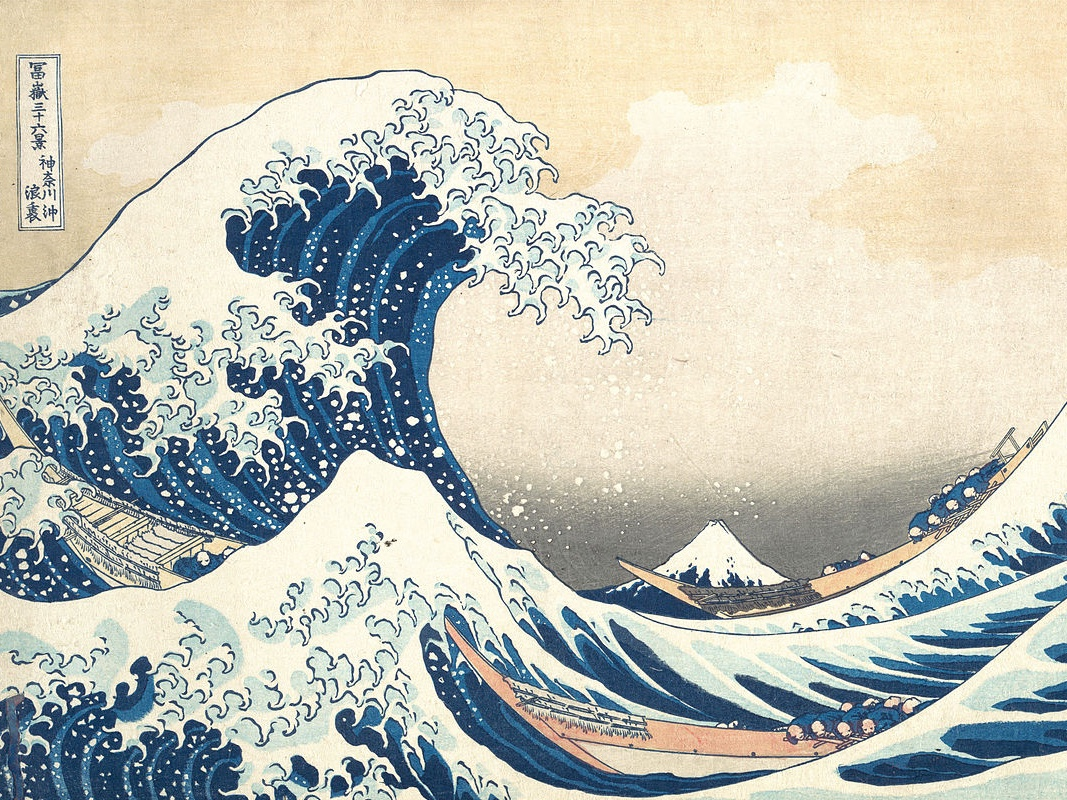
\includegraphics[width= .95\linewidth]{img/kanagawa.jpg}
    \end{center}
\end{frame}

\begin{frame}{Figure with comments}
    \begin{columns}[T] % align columns
    \begin{column}{.62\textwidth}
        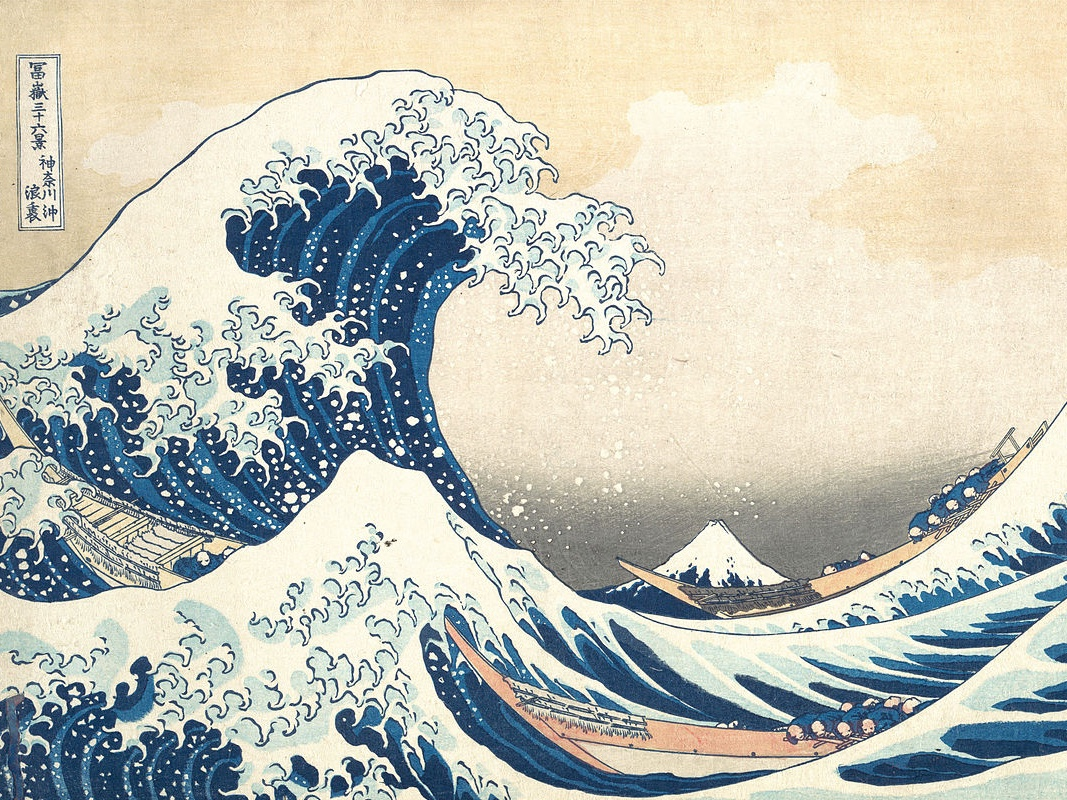
\includegraphics[width= \linewidth]{img/kanagawa.jpg}
    \end{column}%

    \begin{column}{.38\textwidth}
        % Horizontal Bar
        {\color{accent}\rule{\linewidth}{3pt}}
        
        \begin{itemize}[leftmargin=0cm]
            \item Point 1 about the figure to the left. This really only works for 16:9 aspect ratio
            \item Point 2
        \end{itemize}
    \end{column}%
    \end{columns}
\end{frame}


\begin{frame}{Two Columns general}
    \begin{columns}[T] % T = vertical align columns at the top
    \begin{column}{.50\textwidth}
        {\color{accent}\rule{\linewidth}{3pt}}
        Column 1
    \end{column}
    
    \hfill
    
    \begin{column}{.50\textwidth}
        {\color{accent}\rule{\linewidth}{3pt}}
        Column 2
    \end{column}
    \end{columns}
\end{frame}


% --------------------------------------------------
\begin{frame}[allowframebreaks]{References}
    \printbibliography
\end{frame}
% --------------------------------------------------


% --------------------------------------------------
\appendix
% --------------------------------------------------

\begin{frame}{Appendix Slide}\label{appendix1}

    % Adjust Font Size to make table fit
    {\fontsize{9}{10}\selectfont
    
        \begin{table}
            \centering 
            \caption{Summary Statistics}
            \label{appendix_summ_stat}

            \begin{tabularx}{\linewidth}{@{} LCCCCCCC @{}} 
                \hline 
                \hline \\[-1.8ex] 
                Statistic & \multicolumn{1}{c}{N} & \multicolumn{1}{c}{Mean} & \multicolumn{1}{c}{St. Dev.} & \multicolumn{1}{c}{Min} & \multicolumn{1}{c}{Pctl(25)} & \multicolumn{1}{c}{Pctl(75)} & \multicolumn{1}{c}{Max} \\ 
                \hline \\[-1.8ex] 
                rating & 30 & 64.633 & 12.173 & 40 & 58.8 & 71.8 & 85 \\ 
                complaints & 30 & 66.600 & 13.315 & 37 & 58.5 & 77 & 90 \\ 
                privileges & 30 & 53.133 & 12.235 & 30 & 45 & 62.5 & 83 \\ 
                learning & 30 & 56.367 & 11.737 & 34 & 47 & 66.8 & 75 \\ 
                raises & 30 & 64.633 & 10.397 & 43 & 58.2 & 71 & 88 \\ 
                critical & 30 & 74.767 & 9.895 & 49 & 69.2 & 80 & 92 \\ 
                advance & 30 & 42.933 & 10.289 & 25 & 35 & 47.8 & 72 \\ 
                \hline \\

                \multicolumn{8}{p{.8\textwidth}}{\textit{Notes:} Using R base dataframe attitude}
            \end{tabularx} 
            
        \end{table} 
        
    }
    
    \hyperlink{main1}{\beamergotobutton{Back to Main}}
\end{frame}
\end{document}
